\documentclass{article}
\usepackage[utf8]{inputenc}
\usepackage{graphicx}
\usepackage{amsmath}
\usepackage{caption}
\usepackage{subcaption}
\usepackage{amssymb}

%----------------------------MATLAB TEMPLATE -------------------------------------
\usepackage{listings}
\usepackage{color} %red, green, blue, yellow, cyan, magenta, black, white
\definecolor{mygreen}{RGB}{28,172,0} % color values Red, Green, Blue
\definecolor{mylilas}{RGB}{170,55,241}
%-----------------------------------------------------------------------------------------

\title{ECE 8540 Analysis of Tracking Systems \\ 
	Assignment 1}
\author{Vivek Koodli Udupa \\ C12768888}
\date{09/04/2018 }

\begin{document}

%Displaying Title
\begin{titlepage}
\maketitle
\pagenumbering{gobble}% Remove page numbers (and reset to 1)
\end{titlepage}
\pagenumbering{arabic}% Arabic page numbers (and reset to 1)

\section{Aim}
\subsection*{Part 1:} To fit a 2D line to the given five (x , y) data points. Construct the appropriate matrices and solve for the line parameters using the Normal Equations.
\subsection*{Part 2:} Follow the same steps as Part 1 but include an extra point  (8 , 14). Find out what happens.
\subsection*{Part 3:} Fit a model for the data set that contains the data of 3398 meals eaten by 83 different people. Using the normal equations, formulate the matrices and fit that model to the data. 

\section{Execution}
\subsection*{Part 1 and Part 2}
The Dataset for Part 1: (5 , 1); (6 , 1); (7 , 2); (8 , 3); (9 , 5). \\
The Dataset for Part 2: (5 , 1); (6 , 1); (7 , 2); (8 , 3); (9 , 5); (8 , 14). 

\begin{figure}[h!]
\centering
\begin{minipage}{0.5\textwidth}
	\centering
	\includegraphics[scale = 0.40]{Part1_Dataplot.eps}
		\captionof{figure}{ Plot of Dataset 1}
		\label{fig:Data1}
\end{minipage}%
\begin{minipage}{0.5\textwidth}
	\centering
	\includegraphics[scale = 0.40]{Part2_Dataplot.eps}
	\captionof{figure}{ Plot of Dataset 2}
	\label{fig:Data2}
\end{minipage}
\end{figure}

\quad \\ %To remove the spacing before "Looking"
Looking at the plot in Figure~\ref{fig:Data1} and Figure~\ref{fig:Data2}, a straight line of the form \\  y = ax + b seems to be a good fit.  \\
\newpage
\noindent Formulating the matrices: \\

%A Matrix
\begin{equation}
A = 
	\begin{bmatrix}
		x_1 & 1 \\
		..   & ..  \\
		..   & ..  \\
		x_N & 1 \\
	\end{bmatrix}
\end{equation}
\\
%B Matrix
\begin{equation}
	x = 
	\begin{bmatrix}
	a \\
	b \\
	\end{bmatrix}
\end{equation}
\\
%Unknowns matrix
\begin{equation}
	b = 
	\begin{bmatrix}
	y1 \\
	.. \\
	.. \\
	y_N\\
	\end{bmatrix}
\end{equation} \\
A is a N x M Matrix, \\
where N = 5 ( Number of data points ) and M = 2 ( Number of unknowns ) \\
\\
Filling in the matrices with appropriate values for Data set 1, we get: \\

\[
A=
  \begin{bmatrix}
	
     5 & 1 \\
     6 & 1 \\
     7 & 1 \\
     8 & 1 \\
     9 & 1 \\    
  \end{bmatrix}
\]
\\
\[
b=
  \begin{bmatrix}
	1 \\
     	1 \\
     	2 \\
     	3 \\
     	5 \\    
  \end{bmatrix}
\]
\\
\[
x\_u=
  \begin{bmatrix}
	a \\
	b \\    
  \end{bmatrix}
\]

With the above matrices, we can find x\_u as :
\begin{equation}
	x\_u = (A^T A)\textsuperscript{-1}A^Tb
\end{equation}

Using MATLAB for calculations, we get  \\
\[
x\_u = 
	\begin{bmatrix}
	-1.00 \\
	-4.60
	\end{bmatrix}
\]

\noindent Similarly formulating the matrices for data-set 2, we get: \\
\[
A2=
  \begin{bmatrix}
	
     5 & 1 \\
     6 & 1 \\
     7 & 1 \\
     8 & 1 \\
     9 & 1 \\
     8 & 14 \\
   \end{bmatrix}
\]
\\
\[
b2=
  \begin{bmatrix}
	1 \\
     	1 \\
     	2 \\
     	3 \\
     	5 \\  
     	14 \\  
  \end{bmatrix}
\]
\\
\[
x\_u2=
  \begin{bmatrix}
	a \\
	b \\    
  \end{bmatrix}
\]

Using MATLAB for calculations, we get  \\
\[
x\_u2 = 
	\begin{bmatrix}
	 1.8154 \\
   	-8.6769
	\end{bmatrix}
\]

\noindent Now, we can fit a line of the form 
\begin{align*}
	y &= a * x + b  ;\quad  \text{where } 
 	a = x\_u(1,1)  \text{ and } 
 	b = x\_u(2,1) 
\end{align*}
(Note: Similar line fit is calculated for data set 2 with its respective values )

\begin{figure}[h]
\centering
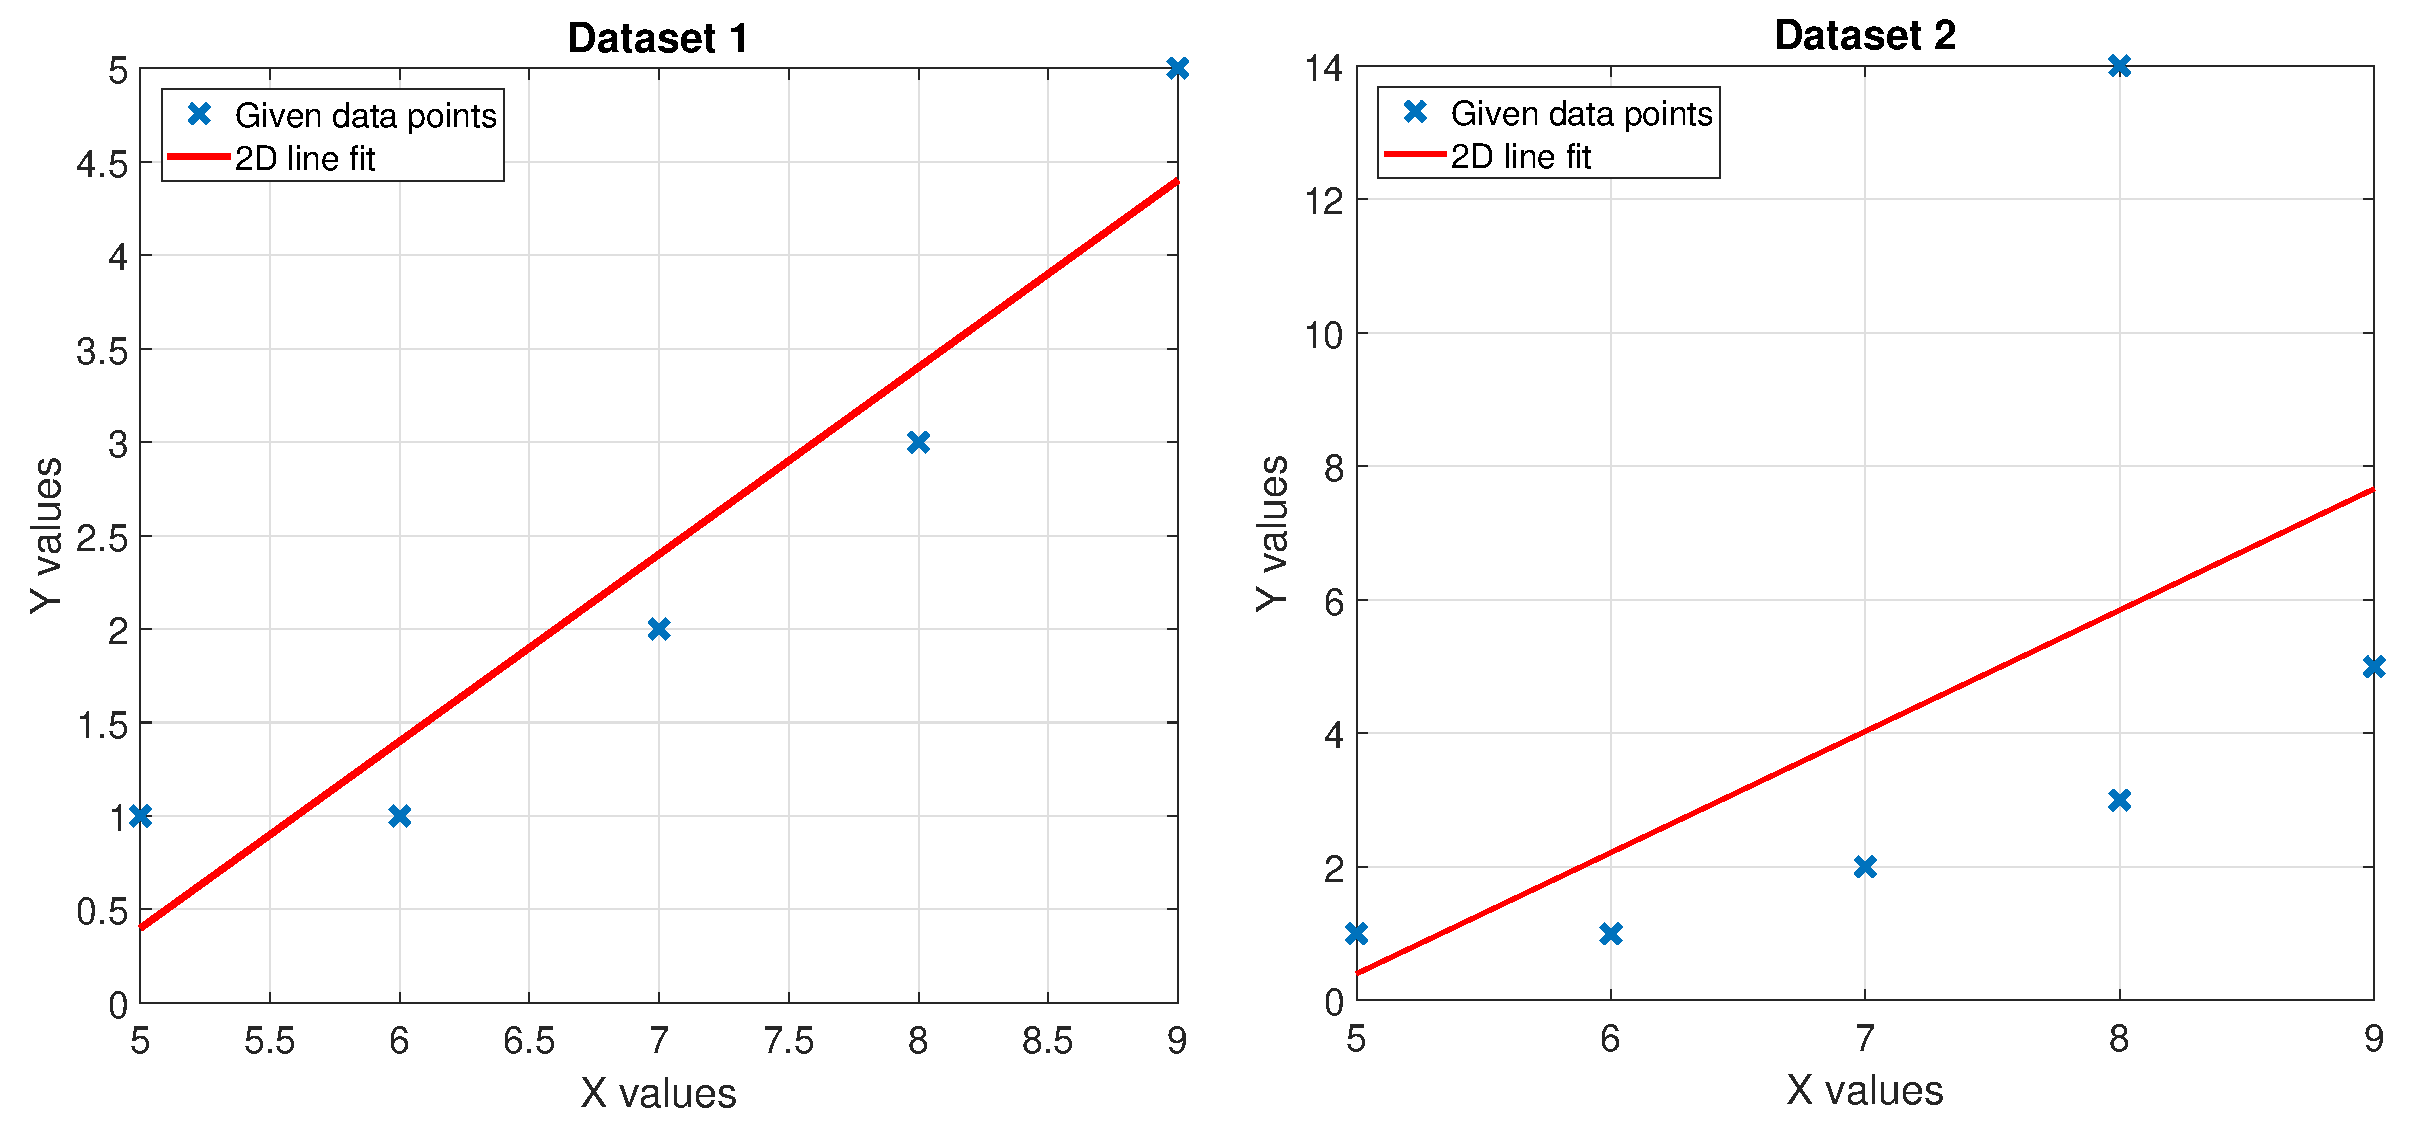
\includegraphics[width=\textwidth]{Fit.eps}
\caption{Dataset 1 and Dataset 2 Line Fit}
\label{fig:Fit}
\end{figure}
Figure~\ref{fig:Fit} shows the dataset plot with fitted line.
\newpage

\subsection*{Part 3}
The data for part 3 of the lab contains 3,398 meals eaten by 83 different people. It has 4 columns and they represent the following:
\begin{enumerate}
	\item{Participant ID}
	\item{Meal ID}
	\item{Number of Bites taken in the meal}
	\item{Number of Kilo calories consumed}
\end{enumerate}

\begin{figure}[h]
\centering
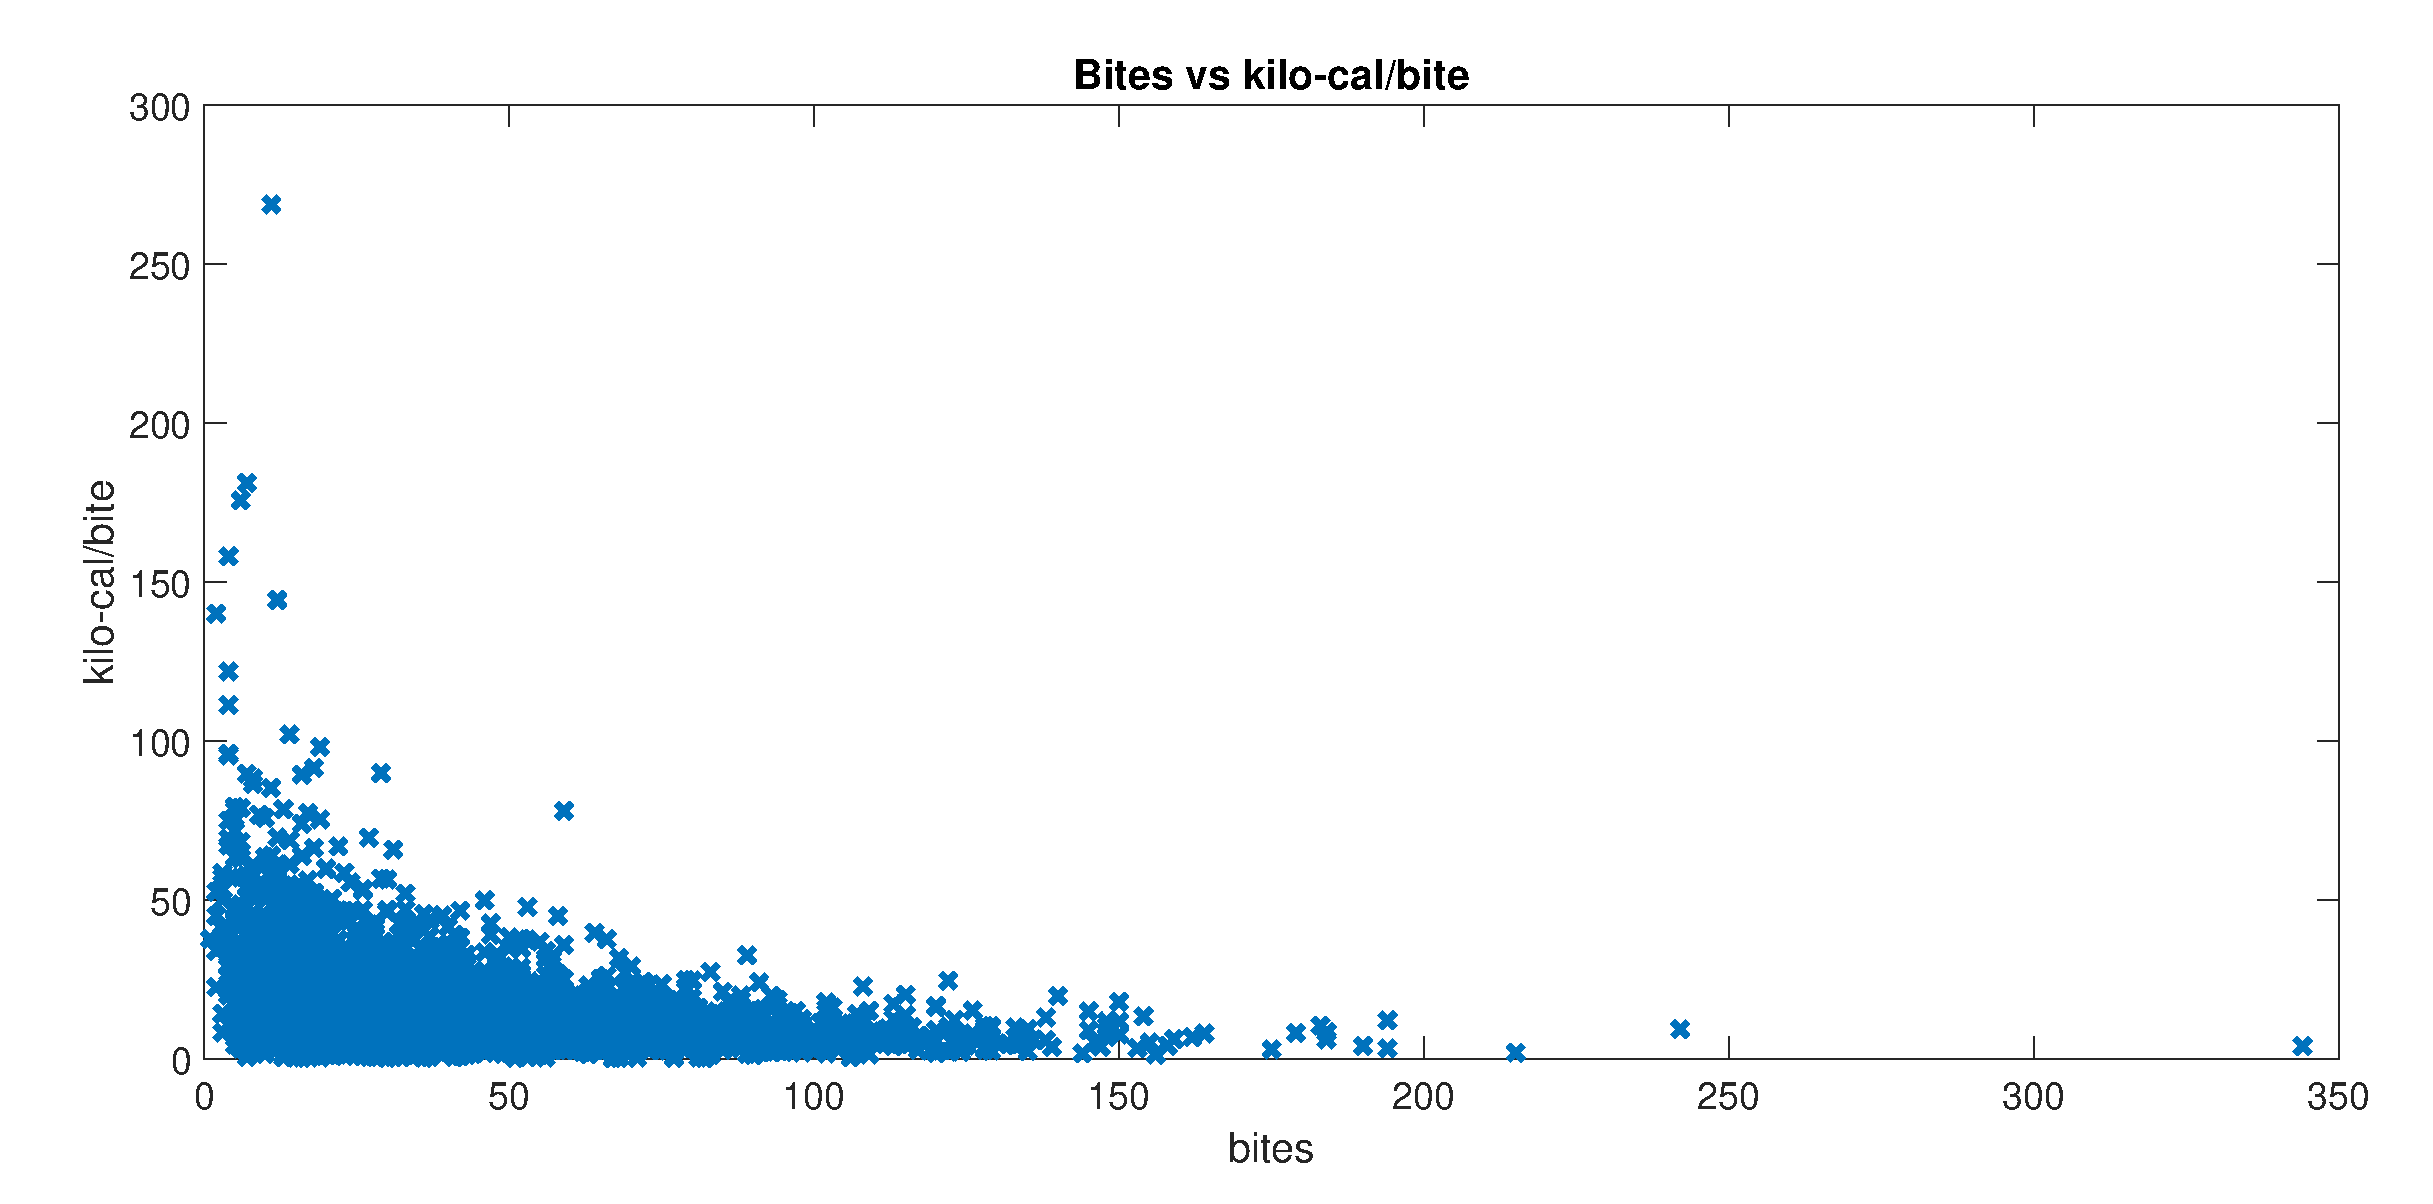
\includegraphics[width=\textwidth]{Part3_Dataplot.eps}
\caption{Plot of bites VS Kilo-calories per bite }
\label{fig:bites}
\end{figure}
\noindent
Figure~\ref{fig:bites} shows the plot of kilo-calories consumed per bite against the total number of bites taken. \\
The values of the Y-axis is obtained by dividing Column 4 / Column 3 from the given data-set. The values of X-axis are from Column 3 of the Data-set. \\
\quad \\
The distribution of the given data as shown in Figure~\ref{fig:bites} is concentrated near the origin and scarce at the farther end of X and Y axes. \\

\noindent
We will try to fit a line using the same methods as we used for Part 1 and Part 2, we get: \\
\[
x\_u3 =
\begin{bmatrix}
	-0.1771 \\
   	23.4417
\end{bmatrix}
\]
\newpage

\begin{figure}[h]
\centering
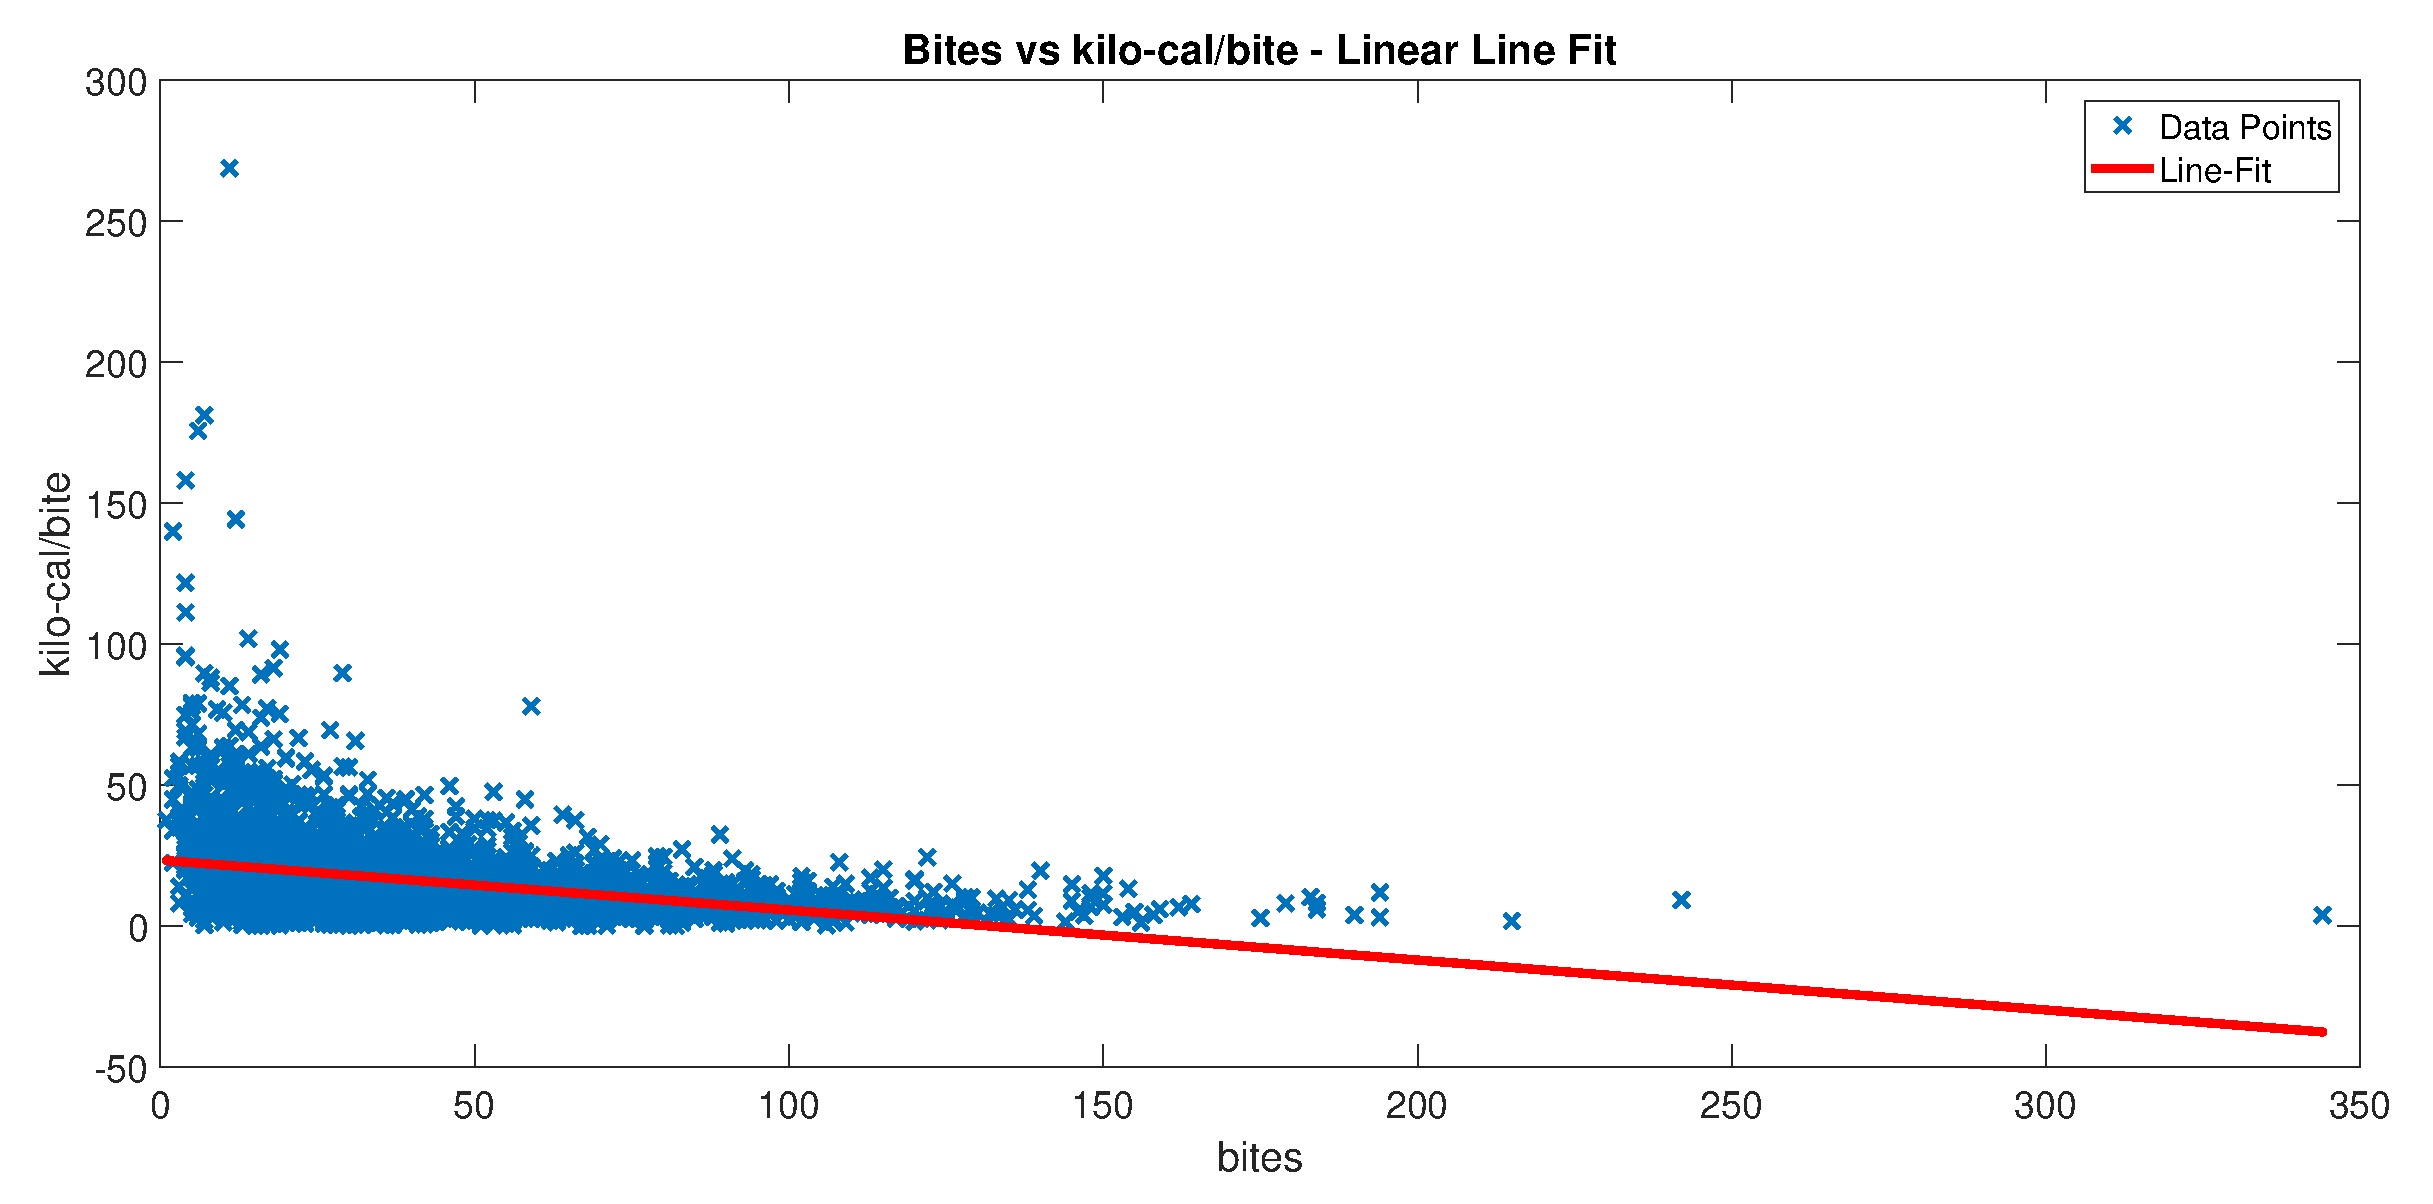
\includegraphics[width=\textwidth]{Part3_line.eps}
\caption{Line fit for Part 3 Data-set }
\label{fig:LineFit3}
\end{figure}

\noindent
Fitting a line using the values obtained gives us the result shown in Figure~\ref{fig:LineFit3}. The line extends way ahead along the X-axis and has high error values for points in the Y-axis. The linear line is not a great fit for this data set.  \\

\noindent
Power fit with the equation of the form $y = ax^b$ seems to be a better option.\\
Here we have two unknowns ( a and b ).  We have to model the above equation. 

\begin{align}
	y &= ax^b \\
	log( y ) &= log( ax^b )  \\
	log( y ) &= log( a ) + log( x^b ) && \because [ log(mn) = log(m) + log(n) ] \\
	log( y ) &= log( a ) + blog( x ) && \because [log(m^n) = n log( m ) ] 
\end{align}
Above equation is of the form
\begin{align}
	v &= k + bu && \text{where} \\
	v &= log(y) \\
	k &= log(a) \\
	u &= log(x)
 \end{align}
\noindent 
Formulating the Matrices: \\
%A Matrix
\begin{equation}
A = 
	\begin{bmatrix}
		log(x_1) & 1 \\
		..   & ..  \\
		..   & ..  \\
		log(x_N) & 1 \\
	\end{bmatrix}
\end{equation}
\\
%B Matrix
\begin{equation}
	x = 
	\begin{bmatrix}
	b \\
	a \\
	\end{bmatrix}
\end{equation}
\\
%Unknowns matrix
\begin{equation}
	b = 
	\begin{bmatrix}
	log(y1) \\
	.. \\
	.. \\
	log(y_N)\\
	\end{bmatrix}
\end{equation} \\

\noindent
Using the solution to the normal equations i.e. 
\begin{equation}
	x = (A^T A)\textsuperscript{-1}A^Tb
\end{equation}

\noindent We get the values of the unknowns as a = 57.7128 and b = -0.4601.  Now we can plot the power fit. 

\begin{figure}[h]
\centering
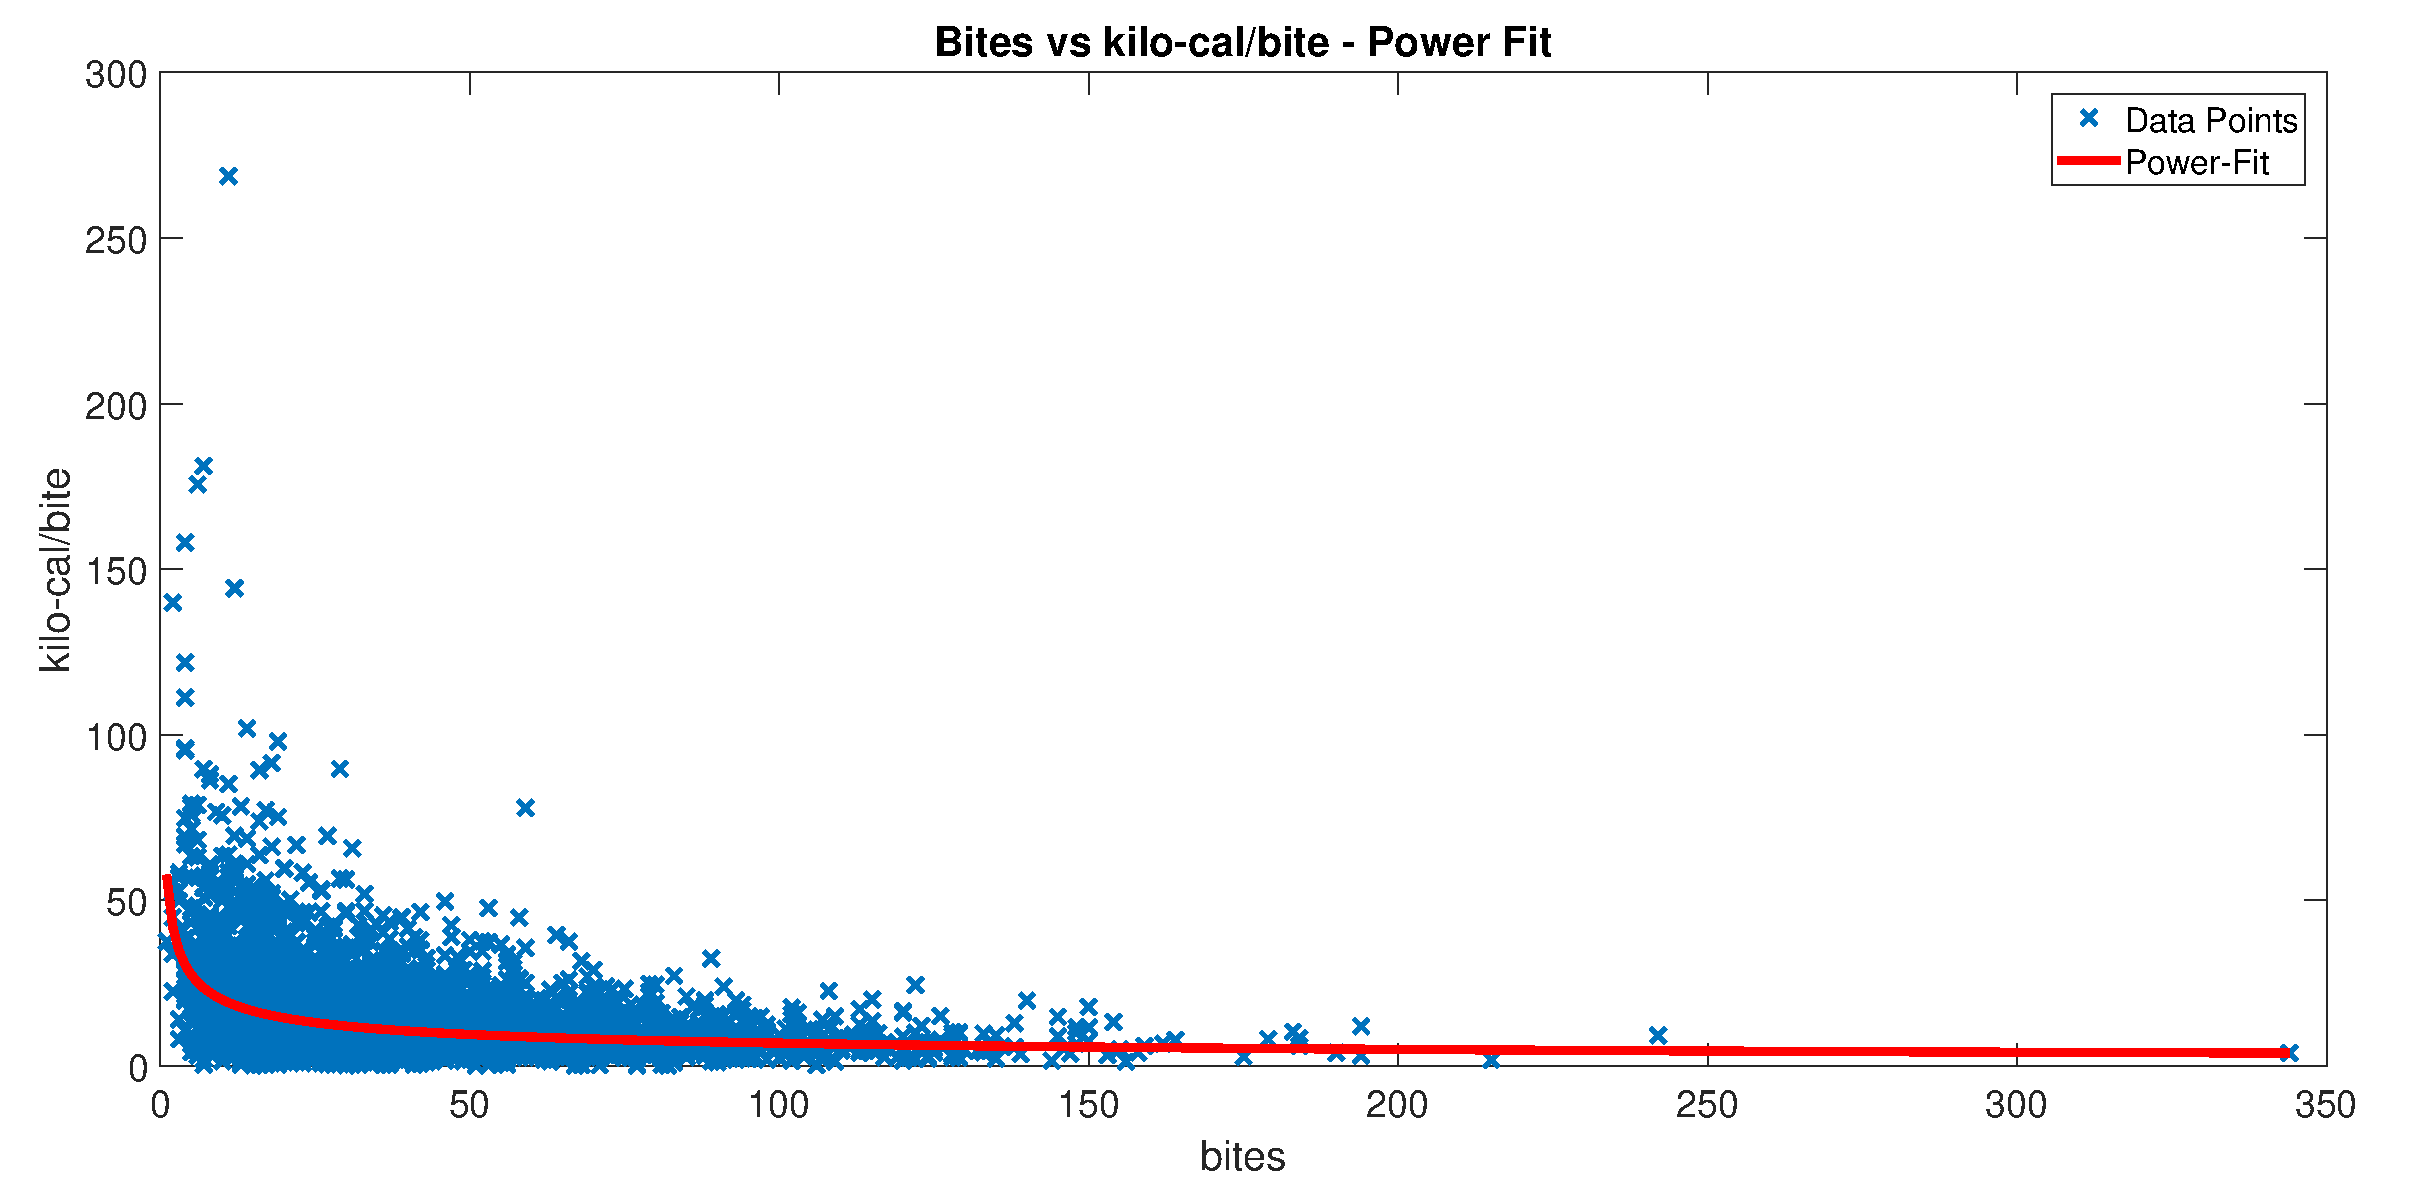
\includegraphics[width=\textwidth]{powerfit.eps}
\caption{Power Fit}
\label{fig:powerfit}
\end{figure}

\section{Conclusion}
\subsection*{Part 1 and Part 2}
The raw data-points given for Part 1 and Part 2 of the lab were plotted using MATLAB.  Appropriate matrices for solving the line parameters using Normal Equations were constructed an the line fit was plotted. Figure~\ref{fig:Data1} and Figure~\ref{fig:Data2} represents the raw data plot and Figure~\ref{fig:Fit} shows the line fit. \\
Due to the addition of an extra point (8 , 14), which has a high y-axis value, the y-intercept of the line fit approximately doubled. The unknowns for Part 1 are \textbf{a = -1.00 and b = -4.60} and the unknowns for Part 2 are \textbf{a = 1.8154 and b = -8.6769}. \\

\subsection*{Part 3}
For Part 3 of the lab, the data-set named "83people-all-meals.txt" which was given in the website was imported into MATLAB as a table and then converted into array using the inbuilt function "table2array". Having the data as an array eases the calculation process. Kilo-calories per bite VS bites taken were plotted. \\
Line model was used initially to fit the data. It did not fit well. Later on Power model of the form $y = ax^b$ was used, which seems to be a better fit than the Line model. Figure~\ref{fig:LineFit3} and Figure~\ref{fig:powerfit} represent the Line model and power model fit respectively. \\
\quad \\
All calculations were performed on MATLAB and the code has been attached in the appendix. 

%----------------------------------------------MATLAB LISTING TEMPLATE-------------------------

\lstset{language=Matlab,%
    %basicstyle=\color{red},
    breaklines=true,%
    morekeywords={matlab2tikz},
    keywordstyle=\color{blue},%
    morekeywords=[2]{1}, keywordstyle=[2]{\color{black}},
    identifierstyle=\color{black},%
    stringstyle=\color{mylilas},
    commentstyle=\color{mygreen},%
    showstringspaces=false,%without this there will be a symbol in the places where there is a space
    numbers=left,%
    numberstyle={\tiny \color{black}},% size of the numbers
    numbersep=9pt, % this defines how far the numbers are from the text
    emph=[1]{for,end,break},emphstyle=[1]\color{red}, %some words to emphasise
    %emph=[2]{word1,word2}, emphstyle=[2]{style},    
}

\section{Appendix}

\lstinputlisting{asg1.m}
%--------------------------------------------------------------------------------------------------------
\quad \\
\quad \\
\quad \\
\section*{----------------------------END-----------------------------}
\end{document}
